
\section{Problem 1}
\begin{wrapfigure}[10]{R}{0.4\textwidth}
    \begin{center}
      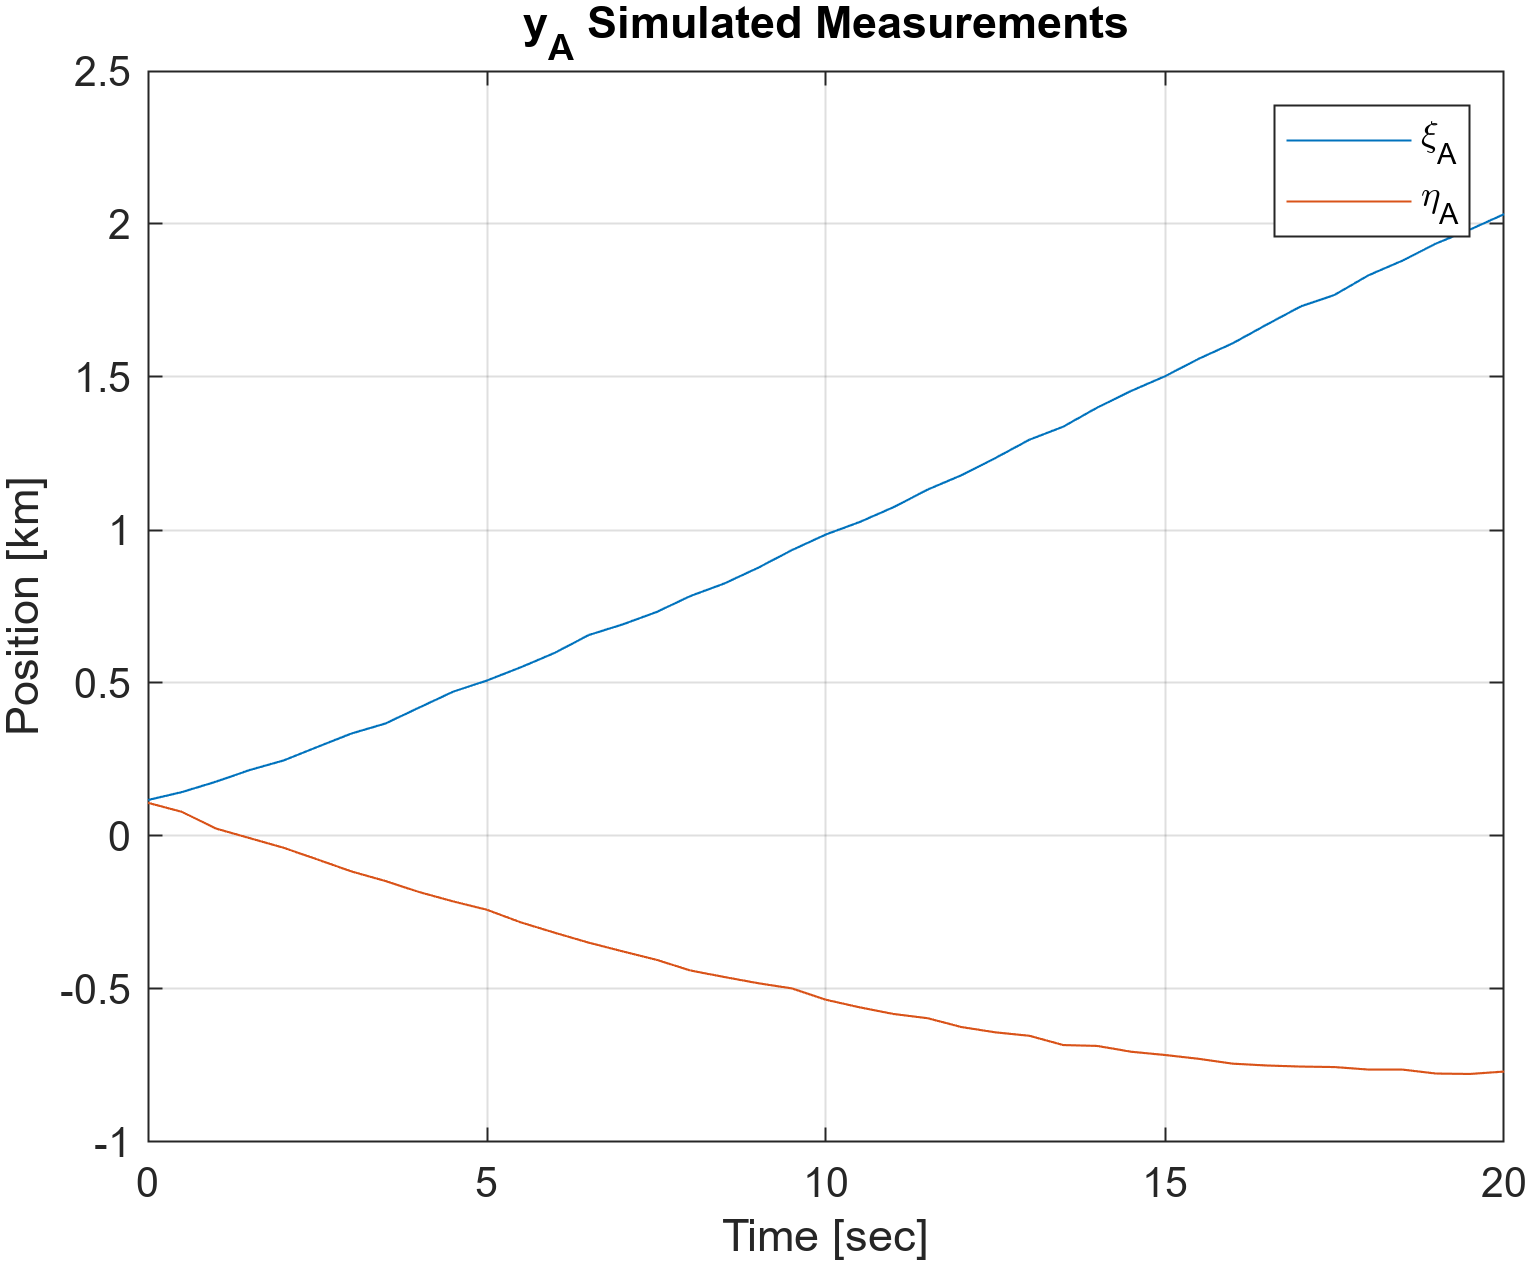
\includegraphics[width=0.8\linewidth]{figs/p2pa.png}
    \end{center}
    \caption{Birds}
\end{wrapfigure}
\lipsum[55]
\subsection{Part A}
%
\begin{remark}[test]
    \lipsum[55]
\end{remark}
%
\lipsum[23]
%
\begin{figure}[h!tbp]
    \centering
    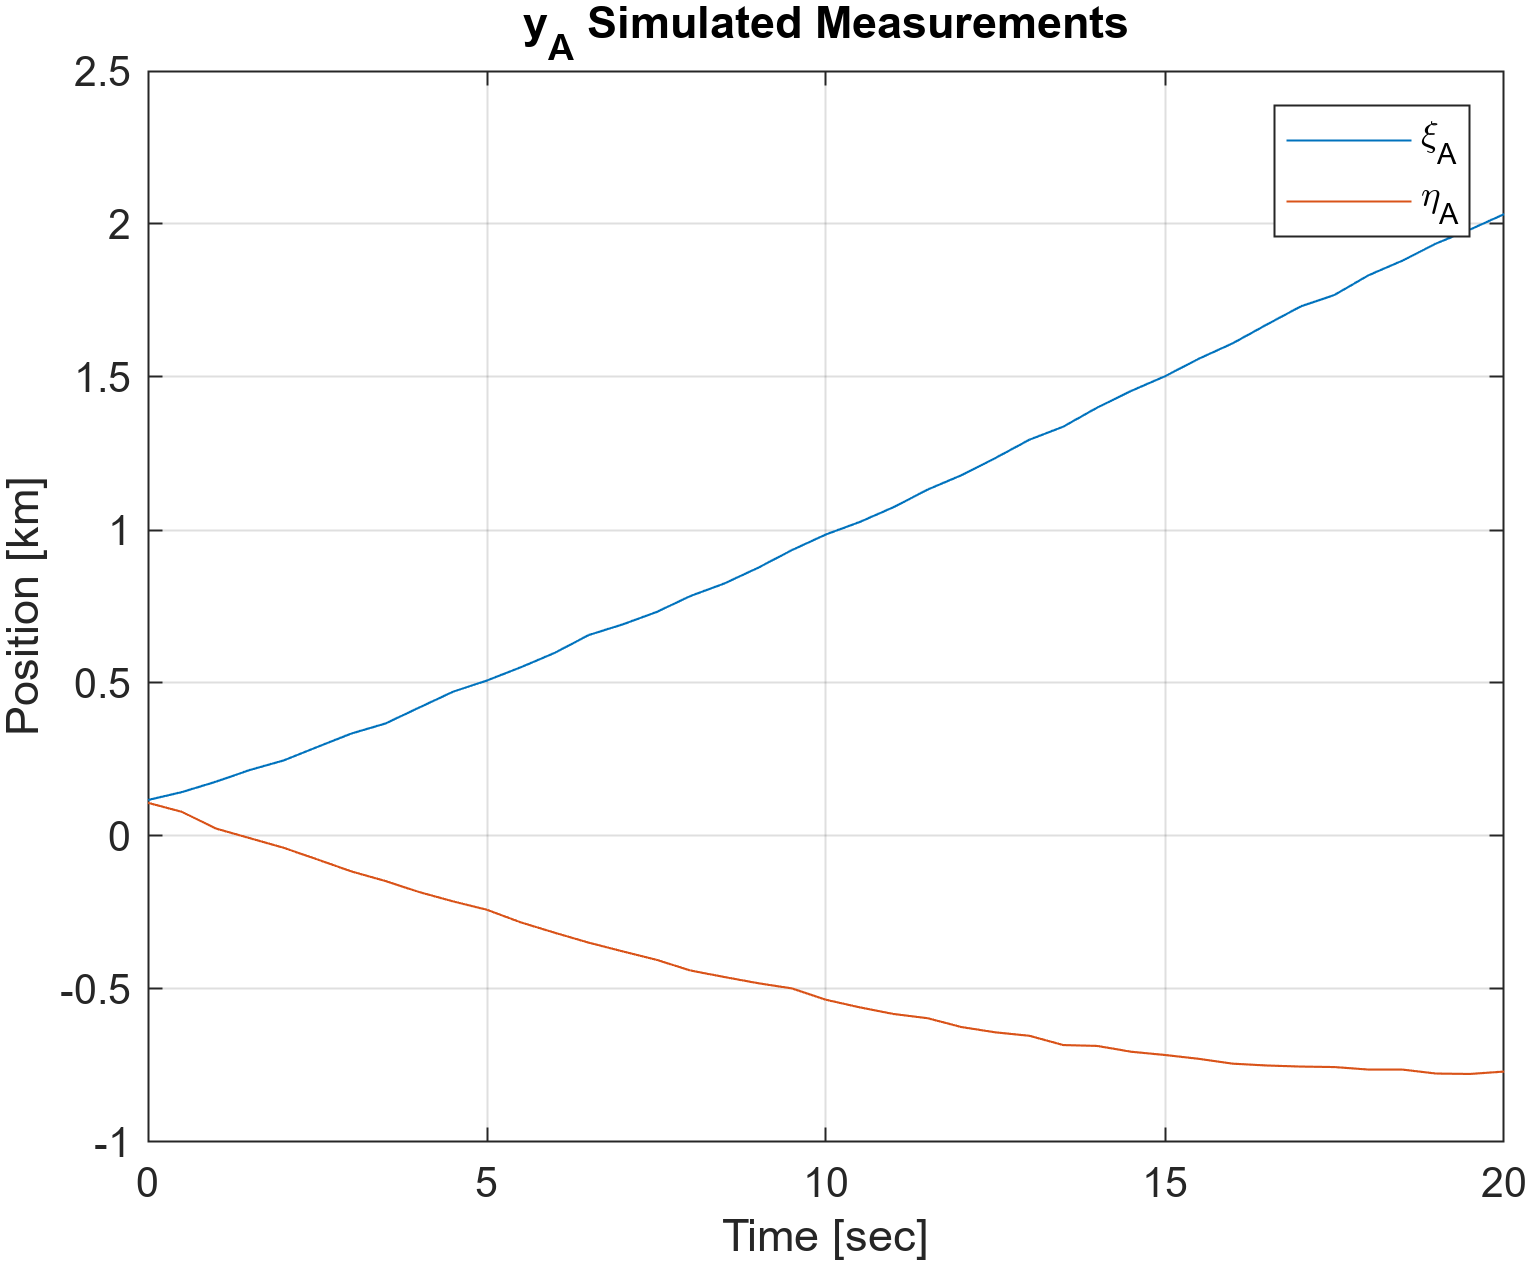
\includegraphics[width=0.6\textwidth]{figs/p2pa.png}
    \caption{20 seconds of simulated measurements}
    \label{fig:p2_a}
\end{figure}
%
\lipsum[26]
%
\begin{definition}[test]
    \lipsum[44]
\end{definition}
%
\lipsum[32]
%
\subsection{Part b}
\begin{theorem}[test]
    \lipsum[2]
\end{theorem}
%
\lipsum[34]
%
\begin{eg}[test]
    \lipsum[36]
\end{eg}
%
\subsection{Code Example}
\begin{minted}{python3}
    import numpy as np
    from sklearn.decomposition import KernelPCA
    from sklearn.datasets import make_classification
    from sklearn.model_selection import GridSearchCV
    import matplotlib.pyplot as plt

    # Step 1: Generate a sample dataset
    X, y = make_classification(n_samples=100, n_features=20, random_state=42)

    # Step 2: Define the hyperparameter grid
    param_grid = {
        'kernel': ['linear', 'rbf', 'poly'],  # Different kernels to test
        'gamma': [0.01, 0.1, 1, 10],  # Only for RBF kernel
        'degree': [2, 3, 4],  # Only for polynomial kernel
    }

    # Step 3: Custom KPCA class to handle kernel-specific parameters
    class CustomKPCA(KernelPCA):
        def __init__(self, kernel='linear', gamma=None, degree=3, n_components=2):
            super().__init__(kernel=kernel, gamma=gamma, degree=degree, n_components=n_components)

        def fit(self, X, y=None):
            if self.kernel != 'rbf':
                self.gamma = None
            if self.kernel != 'poly':
                self.degree = 3
            return super().fit(X)
        
    def custom_score(estimator, X):
        X_transformed = estimator.fit_transform(X)
        explained_variance = explained_variance_score(X, estimator.inverse_transform(X_transformed))
        return explained_variance

    # Step 4: Apply Grid Search to tune hyperparameters
    grid_search = GridSearchCV(CustomKPCA(n_components=2), param_grid, cv=3,scoring = custom_score, verbose=2)
    grid_search.fit(X)

    # Step 5: Get the best model and parameters
    print("Best Parameters:", grid_search.best_params_)
    best_kpca = grid_search.best_estimator_

    # Apply the best KPCA model to the data
    X_kpca = best_kpca.fit_transform(X)

    # Step 6: Visualize the first 2 KPCA components
    plt.scatter(X_kpca[:, 0], X_kpca[:, 1], c=y, cmap='viridis', edgecolor='k', s=50)
    plt.title('KPCA Projection (Best Kernel)')
    plt.xlabel('Principal Component 1')
    plt.ylabel('Principal Component 2')
    plt.show()
\end{minted}